%% Reykjavik University Presentation Template by Joseph T. Foley < foley AT ru DOT is >
\documentclass[aspectratio=169]{rubeamer}
%% Add option "icelandic" to switch sections and labels
%% Add one of these options to change the aspect ratio:
%% 1610 149 54 43 32 which is 16:10 14:9 etc.

%% If you have customizations and packages you use a lot, put them in custom-beamer.sty
%% It will be automatically loaded if it exists
%% I have loaded this with packages and macros I find useful


%%----------- Citations ---------------------------
%% I highly advise using JabRef to manage your .bib files.
%% It can catch a lot of errors early and helps you fill things in.
%% In particular, you probably want to set it to fix line endings to NL only in the preferences.

%%%% Now pick a citation style
%%IEEE citations (just numbers)
%\usepackage[backend=biber, bibencoding=utf8, style=ieee]{biblatex}

%% APA style (author, year) -- need all of these lines
%\usepackage[backend=biber, bibencoding=utf8, style=apa]{biblatex}
%\usepackage[american]{babel}
%\DeclareLanguageMapping{american}{american-apa}  % after biblatex and babel

%% Alphabetic (abbrv-year), more compact
\usepackage[backend=biber, bibencoding=utf8, style=alphabetic]{biblatex}

%% Put your reference library files here. Don't forget to put the .bib
%% extension. If you have multiple people with their own libraries (or
%% are using the Zotero plugin) it is a good idea to have multiple
%% files separated according to some agreement.  This is the divisions the author uses:

\addbibresource{references.bib}%references specific to this paper
\addbibresource{references-ad.bib}%reference related to Axiomatic Design
\addbibresource{references-foley.bib}%references that the author has participated on.  Helpful for writing a CV.
\addbibresource{references-collections.bib}%Due to BibTeX/Biber processing, multi-author books and proceedings must go last if they are used as crossref.


%% ------------------ Graphics ----------------------------%%
\graphicspath{{graphics/}{Graphics/}}
%% This is a list of folders to search for graphics files to include in that order.
%% Each path should be in a {}.  
%% Make sure that the upper/lowercase of the letters matches the folder or
%% you may have weird problems with partners using other operating systems.

\usepackage{datetime}

\newdateformat{monthyeardate}{\monthname[\THEMONTH] \THEYEAR}

%% -----------------Titles and Footers ---------------------%%
%% The abbreviated information goes in the [], the full information in {}
\title[RU Presentation]{Real Time, Autonomous Drone Landing using Only Embedded Processing}
\subtitle[demo]{PhD Thesis Proposal}
\author[Springer]{Joshua Springer}
\institute[RU]{Reykjavík University}
\date[2022]{\monthyeardate\today}%Set this to when you will present

\logo{
\includegraphics[width=1.5cm]{ru-logo}}
\titlegraphic{
\includegraphics[width=2CM]{ru-logo}}

\begin{document}
%----------- titlepage ----------------------------------------------%
\begin{frame}[plain]%plain option gets rid of the footer and the per-page logo
  \titlepage
%  \begin{textblock}{10}(12,4)
%    
\includegraphics[width=0.3\textwidth]{ru-logo}
%  \end{textblock}

\end{frame}

%\rutitleframe{}

%----------- slides ----------------------------------------------%
\begin{frame}
  \frametitle{Introduction}
  How to get help:
  \begin{itemize}
  \item \url{http://tug.ctan.org/macros/latex/contrib/beamer/doc/beameruserguide.pdf}
  \item \url{http://tex.stackexchange.com}  {\it but Caveat Emptor!}\/
  \item \url{http://overleaf.com}
  \item \url{latex@list.ru.is} for template related questions
  \end{itemize}

\end{frame}

\begin{frame}
  \frametitle{Preparing the Presentation}
  \begin{itemize}
  \item Give sources for all pictures and cite information sources e.g. \cite{vossebeld2018customer}
  \item More pictures, less text.
  \item More slides, less time per slide.
  \item 45--60 seconds per slide, no more.
  \item Tell a story (make sure it flows).
  \item Spellcheck!
  \item Freeze any changes at least an hour before you present:  {\em last minute changes confuse the presenters}\/
  \end{itemize}
\end{frame}

\begin{frame}[fragile]%You need the fragile option when you have any sort of verbatim environment
  \frametitle{Dealing with graphics}
  \begin{itemize}
  \item Put them in the \path{graphics/} folder, not where the \url{.tex} is.  This will keep your folders from becoming messy.
  \item Reduce the image sizes to a maximum of 1920$\times$1080 e.g using ImageMagick (\url{https://imagemagick.org}):
\begin{verbatim}
  mogrify -size 1920x1920 *.jpg
\end{verbatim}
    will resize all jpg files in that folder to keep their aspect ratios but have no dimension bigger than 1920.
    \item Give credit and/or a source if the presenters did not create the graphic or photo.
  \end{itemize}
  
\end{frame}

\begin{frame}
  \frametitle{Giving the Presentation}
  \begin{itemize}
  \item Grab the interest of the audience in the first 2 slides
  \item Practice until you can do the slides without looking at them.
    If you must have notes, put them on cards.  Do not read from a page
    nor the slides.  It looks bad.
  \item Scan and look around the audience.
  \item Take a breath or drink instead of saying ``um'' and ``herna''.
  \item Slow down.
  \item Move around: don't just stand at the podium.  Having a pointer really helps with this.
  \end{itemize}
\end{frame}

\begin{frame}
  \frametitle{Citations}
  \begin{itemize}
  \item When in doubt, cite!
  \item Anything in your presentation that you did not personally create should be cited
    \item Use JabRef to manage your \path{.bib} files.
  \item This template uses 4 separate libraries as a demonstration
    \begin{itemize}
    \item \path{references.bib} References for this particular presentation
    \item \path{references-ad.bib} References of a particular subject (Axiomatic Design\cite{suh1990principles,suh2001axiomatic})
      \item \path{references-foley.bib} References from the author's CV library
      \item \path{references-collections.bib} References for multi-author books, proceedings, and other collections.
        They need to be separated so they can be used as ``crossref'' and avoid typing in the information every time.
    \end{itemize}
  \end{itemize}
\end{frame}

\begin{frame}
  \frametitle{Highlighting Stuff}
  
  In this slide, some important text will be
  \alert{highlighted} because it's important.
  Please, don't abuse it. \cite{overleaf:beamer}
  
  \begin{block}{Remark}
    Sample text
  \end{block}
  
  \begin{alertblock}{Important theorem}
    Sample text in red box
  \end{alertblock}
  
  \begin{examples}
    Sample text in green box. The title of the block is ``Examples".
  \end{examples}
\end{frame}

\begin{frame}
  \frametitle{Proof Example: There Is No Largest Prime Number}
  \framesubtitle{The proof uses \textit{reductio ad absurdum}.}
  \begin{theorem}
    There is no largest prime number.
  \end{theorem}
  \begin{proof}
    \begin{enumerate}
    \item<1-| alert@1> Suppose $p$ were the largest prime number.
    \item<2-> Let $q$ be the product of the first $p$ numbers.
    \item<3-> Then $q+1$ is not divisible by any of them.
    \item<1-> But $q + 1$ is greater than $1$, thus divisible by some prime
      number not in the first $p$ numbers.\qedhere
    \end{enumerate}
  \end{proof}
  Source: \cite{wright2017beamer}
\end{frame}

  %% Here is a demonstration of how to place a graphic somewhere arbitrary on the page
  %%\begin{textblock}{width}(X,Y)
  %% width defines a "minipage" for text
  %% X and Y are measured from the top left of the page in centimeters
  %%   or whatever base unit was defined
%  \begin{textblock}{5}(7,2)
%    
\includegraphics[width=\textwidth]{ru-logo}
%  \end{textblock}

%% This is one way to make a graphic in a frame
\begin{frame}
  \frametitle{Graphics demonstration: Þingvellir National Park}
  \begin{figure}
    \centering
    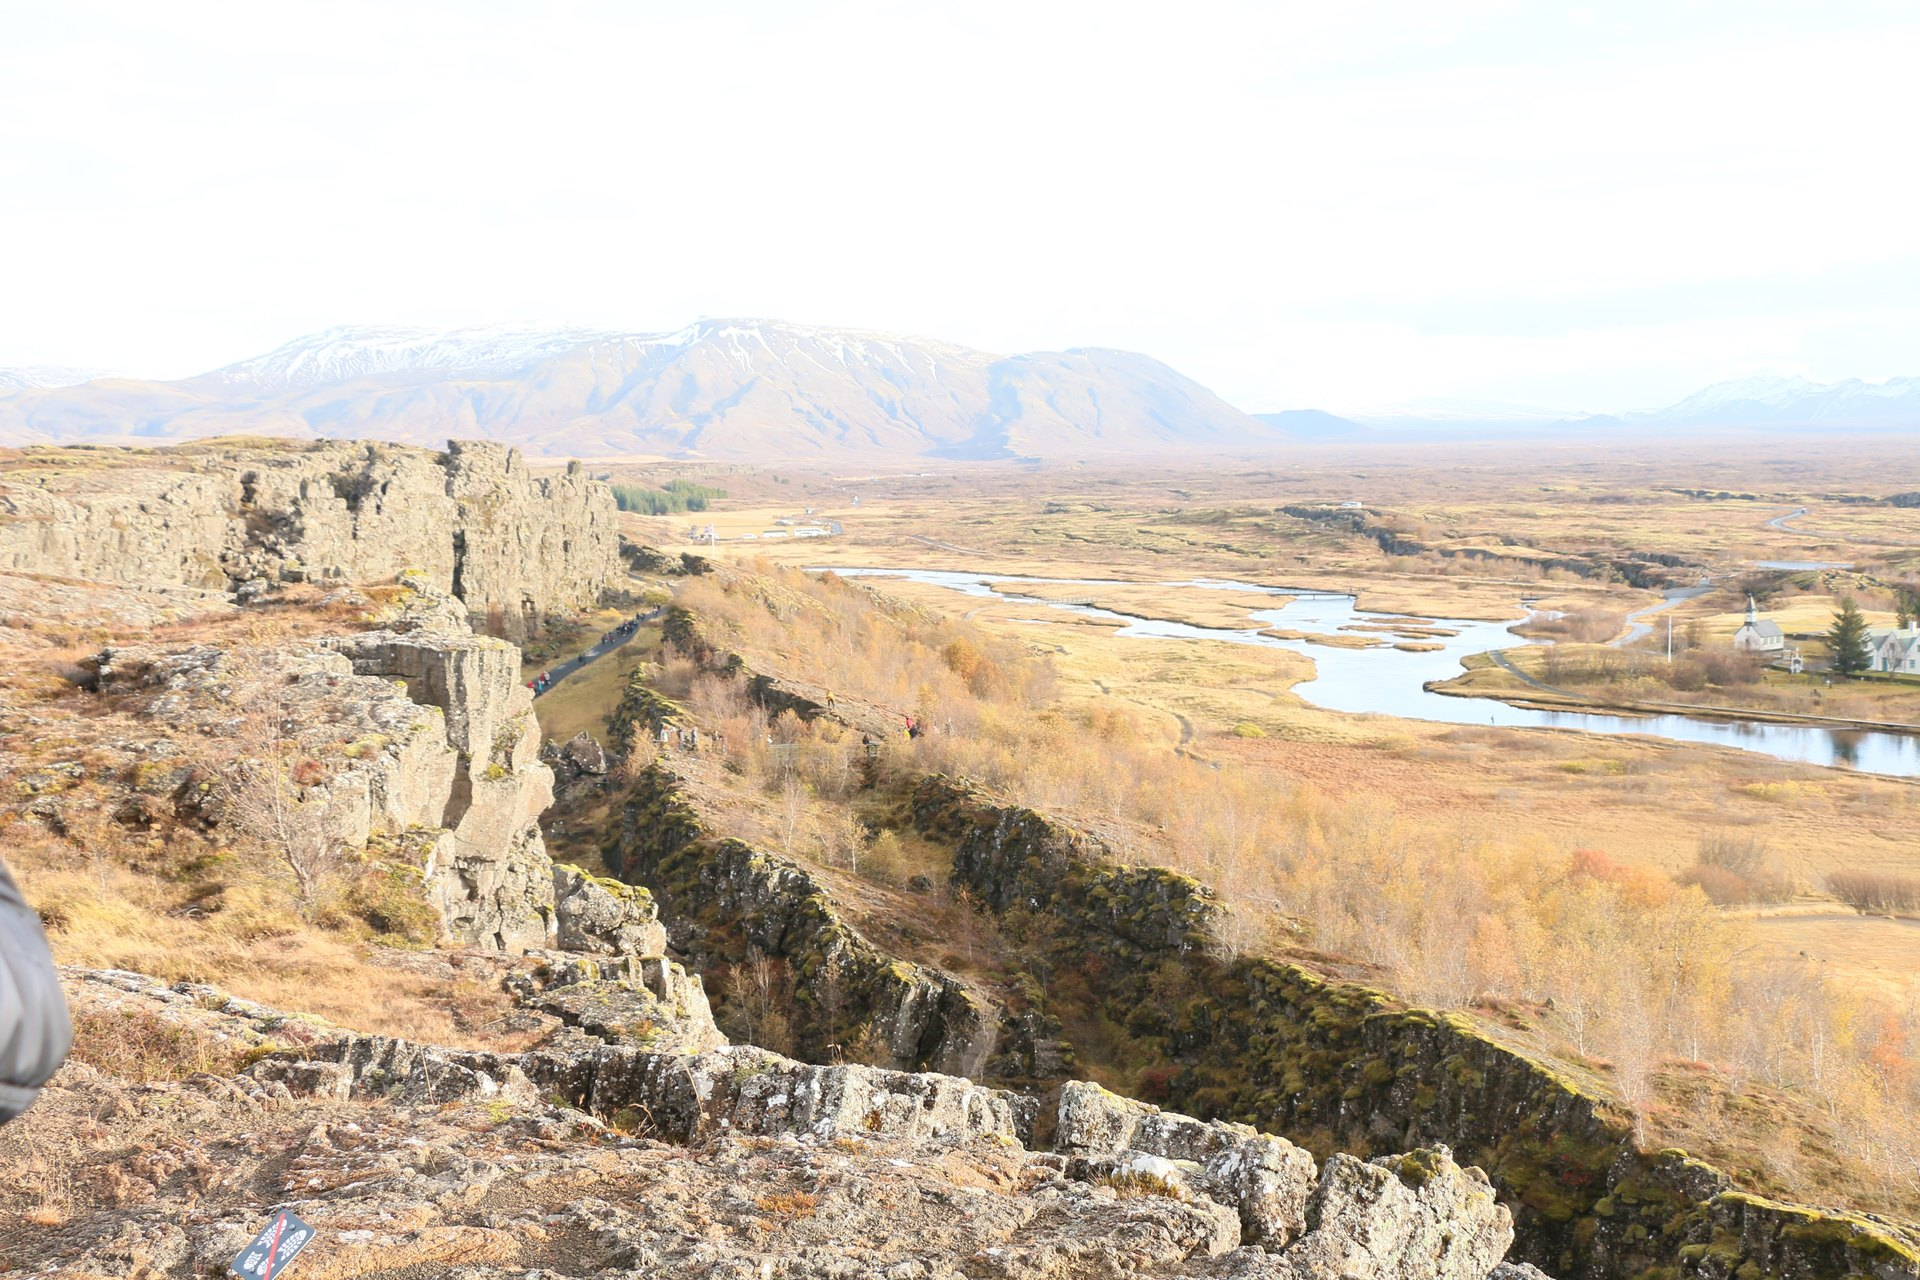
\includegraphics[height=0.8\textheight,width=0.8\textwidth,keepaspectratio]{thingvellir}
    % may have to change the ratios to get it to fit the text nicely
    \caption{The site of the Icelandic parliment meetings of old.  (Credit: J. Foley 2018)}
    \label{fig:thingvellir}
  \end{figure}
\end{frame}

%% in beamer-custom.sty we also create a convenient macro to make it simpler
%% \graphicsframe{Title}{ratio}{filename}{caption text}
%%% You may have to change the ratios to get it to fit the text nicely

\begin{frame}
  \frametitle{Two Column Format:  Strokkur at Geysir}
  \begin{columns}
    \column{0.5\textwidth}
    \begin{itemize}
    \item Hot
    \item Wet
    \item Where we get the English word ``Geyser from.
    \end{itemize}
    \column{0.5\textwidth}
    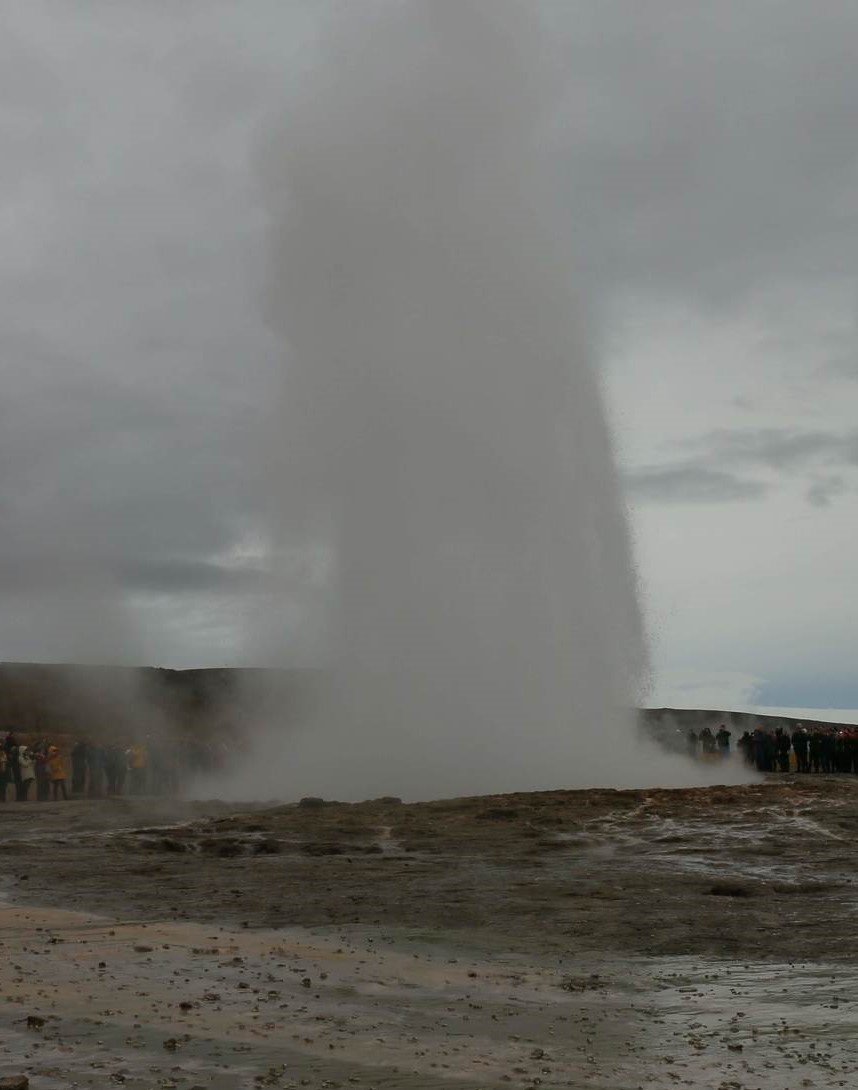
\includegraphics[height=0.75\textheight]{geysir-strokkur-2crop}\\
    Credit: J. Foley 2018
  \end{columns}
\end{frame}

\begin{frame}[allowframebreaks]
  \frametitle{References}
  Thank you for your time.
  Questions?
  \printbibliography{}

\end{frame}

\end{document}
%%%%%%%%%%%%%%%%%%%% TeXStudio Magic Comments %%%%%%%%%%%%%%%%%%%%%
%% These comments that start with "!TeX" modify the way TeXStudio works
%% For details see http://texstudio.sourceforge.net/manual/current/usermanual_en.html   Section 4.10
%%
%% What encoding is the file in?
% !TeX encoding = UTF-8
%% What language should it be spellchecked?
% !TeX spellcheck = en_US
%% What program should I compile this document with?
% !TeX program = pdflatex
%% Which program should be used for generating the bibliography?
% !TeX TXS-program:bibliography = txs:///bibtex
%% This also sets the bibliography program for TeXShop and TeXWorks
% !BIB program = bibtex

%%% Local Variables:
%%% mode: latex
%%% TeX-master: t
%%% End:
